% =========================================================================== %
% Yes. This is a document.

\documentclass[
	english,
	aspectratio=169,
	table
]{beamer}

% =========================================================================== %
% Theme
\usepackage{scrlfile}
	\ReplacePackage{beamerthemeSHUR}{./sty/beamerthemeSHUR}
	\ReplacePackage{beamerinnerthemefancy}{./sty/beamerinnerthemefancy}
	\ReplacePackage{beamerouterthemedecolines}{./sty/beamerouterthemedecolines}
	\ReplacePackage{beamercolorthemechameleon}{./sty/beamercolorthemechameleon}

\usetheme[
	pageofpages=/,
	bullet=circle,
	titleline=true,
	alternativetitlepage=true,
	watermark="",
	watermarkheight=0px,
	watermarkheightmult=0
	]
{SHUR}

% =========================================================================== %
% the usual stuff

\usepackage[utf8]{inputenc}
\usepackage[T1]{fontenc}
\usepackage{babel}
\usepackage{lmodern}
\usepackage{microtype}
\usepackage{csquotes}

\usepackage{tabularx}
\usepackage{booktabs}
\usepackage{multirow}

\usepackage{color, colortbl}
\usepackage{xcolor}
	\definecolor{tabhighlight}{RGB}{230,240,255}
	\definecolor{tabcontrast} {RGB}{200,210,255}

\usepackage{tabto}
\usepackage{xspace}

% math
\usepackage{amsmath}
\usepackage{amssymb}
\usepackage{dsfont}
\usepackage[arrowdel]{physics}
\usepackage{mathtools}
\usepackage{siunitx}

\usepackage{minted}
	\usemintedstyle{friendly}

\usepackage{tikz}
	\usetikzlibrary{positioning}
	\usetikzlibrary{matrix}
	\usetikzlibrary{shapes.geometric}
	\usetikzlibrary{backgrounds}
	\usetikzlibrary{calc}
	\usetikzlibrary{decorations.pathreplacing}
	\usetikzlibrary{arrows}
\usepackage{adjustbox}

\usepackage[most]{tcolorbox}
	\tcbsetforeverylayer
		{colback=cyan!10!white,
		 colframe=cyan!75!black,
		 arc=0pt,
		 outer arc=0pt,
		 parbox=false
		}
	\newtcolorbox{codebox}[1][Code]
		{colback=black!5!white,
		 colframe=blue!40!black,
		 title=#1,
		 leftupper=6mm
		}
	\newtcolorbox{cmdbox}[1][Kommandozeilen-Befehl]
		{colback=black,
		 coltext=white,
		 fontupper=\ttfamily ,
		 colframe=blue!40!black,
		 title=#1,
		 outer arc=0pt
		}
	\newtcolorbox{warnbox}[1][Beachte]
		{colback=black!5!white,
		 colframe=red!40!black,
		 title=#1
		}
	\newtcolorbox{hintbox}[1][Tipp]
		{colback=black!5!white,
		 colframe=green!40!black,
		 title=#1
		}
	\newenvironment{itembox}
		{\begin{tcolorbox}\begin{itemize}}%
		{\end{itemize}\end{tcolorbox}}
	\newtcolorbox{doublebox}[1][.3]
		{righthand width=#1\linewidth,
		 sidebyside,
		 sidebyside gap=6mm,
		 sidebyside align=center,
		 lower separated=false}
	
%==============================================================================%
% GLOBAL MACROS

\newcommand*{\eg}{e.\,g. }
\newcommand*{\ie}{i.\,e. }

\newcommand{\Thus}{\ensuremath{\Rightarrow}\xspace}
\newcommand{\thus}{\ensuremath{\rightarrow}\xspace}

\newcommand*{\tabcrlf}{\\ \midrule}			% actually still allows for optional argument

\newcommand*{\inPy}[1]{\mintinline{python3}{#1}}

% =========================================================================== %

\author{Stefan Hartinger}
\title{Programming in Python}
\subtitle{Part 13: The MatPlotLib (II)}
\institute{University Regensburg, Department of Theoretical Physics}
\date{Winter Term 2021/22}

% =========================================================================== %

\begin{document}
% =========================================================================== %

\begin{frame}[t,plain]
\titlepage
\end{frame}

% =========================================================================== %

\begin{frame}{Recap: Basic Plots}
%
\begin{columns}[T]
\column{.5\linewidth}
\begin{itemize}
\item \texttt{plt.plot}
	\begin{itemize}
	\item Takes two iterables, creates xy-plot \emph{in memory}
	\item Optional arguments for colour, markers, linetype, label
	\end{itemize}
\item \texttt{plt.show}
\item \texttt{plt.title}, \texttt{plt.xlabel}, \texttt{plt.ylabel}, \texttt{plt.legend}, \texttt{plt.grid}
\item \texttt{plt.xscale}, \texttt{plt.yscale}, \texttt{plt.xlim}, \texttt{plt.ylim}
\end{itemize}
%
\column{.5\linewidth}
\begin{itemize}
\item Bar Plots (\texttt{plt.bar} and \texttt{plt.barh})
\item Pie Plots (\texttt{plt.pie})
\item Stackplots (\texttt{plt.stackplot})
\item Scatterplots (\texttt{plt.scatter})
\item Quiver Plots (\texttt{plt.quiver})
\item ... and some more
\end{itemize}
\end{columns}
%
\begin{center}
	\emph{Any Questions?}
\end{center}
%
\end{frame}

% =========================================================================== %

\begin{frame}[fragile]{Chapter 10}
%
\begin{itemize}
\item Multiplots
\item Object Oriented Approach
\item 3D Plots
\item Saving Plots into Files
\end{itemize}
%
\end{frame}

% =========================================================================== %

\begin{frame}[fragile]{Multiplots}
%
\begin{itemize}
\item Multiple plots in one window
\item Command \texttt{plt.subplot}
	\begin{itemize}
	\item Defines a grid and selects the \enquote{active plot}
	\item Three Parameters: rows, columns, ID
	\item Subsequent commands affect that grid node
	\end{itemize}
\item Shortcut
	\begin{itemize}
	\item One parameter: \inPy{int rci}
	\item Each digit represents one of rows, columns, ID
	\end{itemize}
\item Optional Parameters
	\begin{itemize}
	\item \texttt{polar} (\inPy{bool}) -- draw polar plots
	\item \texttt{sharex} and \texttt{sharey} (\texttt{Axes} object -- see later) -- use same coordinate settings as other plot
	\end{itemize}
\end{itemize}
%
\end{frame}

% =========================================================================== %

\begin{frame}[fragile]
%
\begin{center}
%
\begin{codebox}[\raggedright Example: Lissajous I, width=.6\linewidth, nobeforeafter, equal height group = grpXmpLissajous]
\begin{minted}[linenos, fontsize=\scriptsize]{python3}
import math
import matplotlib.pyplot as plt

X = [x / 100 for x in range(628)]
Y = [math.sin(3 * x) for x in X]

plt.figure( figsize=(4,8) )
plt.suptitle("Lissajous-Figures")

plt.subplot(211)
plt.title("Cartesian")
plt.plot(X, Y)

plt.subplot(212, polar=True)
plt.title("Polar")
plt.plot(X, Y)

plt.show()
\end{minted}
\end{codebox}
%
\begin{tcolorbox}[title={\raggedright Output: Lissajous I}, width=.30\linewidth, nobeforeafter, equal height group = grpXmpLissajous]
	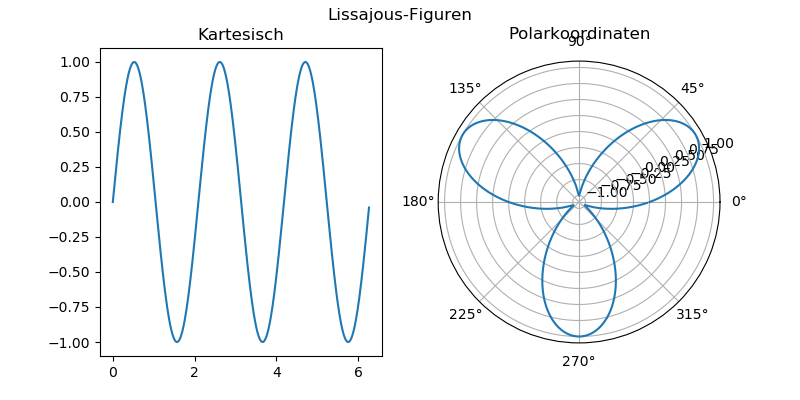
\includegraphics[width=\linewidth]{./gfx/plt-Lissajous}
\end{tcolorbox}
%
\end{center}
%
\end{frame}

% =========================================================================== %

\begin{frame}[fragile]{The Object-Oriented Approach to MatPlotLib/PyPlot}
%
\begin{itemize}
\item Idea: plots and the elements thereof are objects
\item Allows more comfortable/intuitive composition of plots
\item Dynamic evolution of plots (\eg on trigger, zoom in)
\item Primary objects: \texttt{Figure} and \texttt{AxesSubplot}
	\begin{itemize}
	\item \texttt{Figure}: window containing the plots
	\item \texttt{AxesSubplot}: rectangular region in the window where a plot can be placed
	\item Get these objects via \texttt{fig = plt.figure()} and \texttt{ax = fig.add\_subplot()}
	\end{itemize}
\item All objects provide methods for changing them
	\begin{itemize}
	\item E.\;g. \texttt{AxesSubplot}: \texttt{plot}, \texttt{bar}, \texttt{pie}, ...
	\item E.\;g. \texttt{Figure}: \texttt{suptitle}, \texttt{add\_subplot}, \texttt{show}
	\end{itemize}
\item \texttt{show} behaves differently
	\begin{itemize}
	\item \texttt{plt.show()} shows all figures at once, waits till all are closed
	\item \texttt{fig.show()} shows only the figure \texttt{fig}
	\end{itemize}
\end{itemize}
%
\end{frame}

% =========================================================================== %

\begin{frame}[fragile]
%
\begin{codebox}[Example: Lissajous II]
\begin{minted}[linenos, fontsize=\scriptsize]{python3}
import math
import matplotlib.pyplot as plt

X = [x / 100 for x in range(628)]; Y = [math.sin(3 * x) for x in X]

fig = plt.figure(figsize=(4,8))
fig.suptitle("Lissajous-Figures")

crt = fig.add_subplot(1, 2, 1)
crt.set_title("Cartesian")
crt.plot(X, Y)

pol = fig.add_subplot(1, 2, 2, projection="polar")
pol.set_title("Polar")
pol.plot(X, Y)

fig.show()
print("This will be printed while the plots are already portrayed (show does not wait)")
input()
\end{minted}
\end{codebox}
%
\end{frame}

% =========================================================================== %

\begin{frame}[fragile]{Gridspecs}
%
\begin{itemize}
\item Refined control where to place subplots
\item Grid structure where you can \enquote{select} multiple cells
\item Get via \texttt{gs = fig.add\_gridspec(rows, columns)}
\item Use when creating a new subplot: \inPy{ax = fig.add_subplot(gs[...])}
	\begin{itemize}
	\item Index can be a \inPy{tuple} of \inPy{int}s: \texttt{gs[row, column]} ...
	\item ... or a \inPy{tuple} of \inPy{slice}s: \inPy{gs[row_start : row_end, column]}
	\end{itemize}
\end{itemize}
%
\end{frame}

% =========================================================================== %

\begin{frame}
%
\begin{tcolorbox}[title=2D Normal Distribution]
\begin{center}
	\begin{minipage}{.45\linewidth}
	\includegraphics[width=\linewidth]{./gfx/plt-gauss2d}	
	\end{minipage}
	\begin{minipage}{.5\linewidth}
	\begin{itemize}
	\item 3$\times$3 grid
	\item scatterplot: 2$\times$2 tile in the grid, beginning at coordinate (0, 0)
	\item x-histogram: 2$\times$1 tile in the grid, beginning at coordinate (2, 0)
	\item y-histogram: 1$\times$2 tile in the grid, beginning at coordinate (0, 2)
	\item empty tile at coordinate (2, 2)
	\end{itemize}
	\end{minipage}
\end{center}
\end{tcolorbox}
%
\end{frame}

% =========================================================================== %

\begin{frame}[fragile]
%
\begin{codebox}[Code: 2D Normal Distribution ...]
\begin{minted}[linenos, fontsize=\scriptsize]{python3}
import random
import matplotlib.pyplot as plt

N      = 1000
X      =   50; sigmaX =    5
Y      =   40; sigmaY =   10
dataX = [random.gauss(X, sigmaX) for _ in range(N)]
dataY = [random.gauss(Y, sigmaY) for _ in range(N)]

fig = plt.figure(figsize=(8, 8))
gs  = fig.add_gridspec(3, 3)

fig.suptitle("2D Normal Distribution")
fig.subplots_adjust(wspace=0.2, hspace=0.3)  # set spacing between subplots

axScatter = fig.add_subplot(gs[0:2, 0:2])
axScatter.set_xlim(0, 100)
axScatter.set_ylim(0, 100)
axScatter.set_xlabel("x")
\end{minted}
\end{codebox}
%
\end{frame}

% =========================================================================== %

\begin{frame}[fragile]
%
\begin{codebox}[... continued]
\begin{minted}[linenos, firstnumber=last, fontsize=\scriptsize]{python3}
axHistX   = fig.add_subplot(gs[ 2 , 0:2], sharex=axScatter)
axHistY   = fig.add_subplot(gs[0:2,  2 ], sharey=axScatter)

axScatter.scatter(dataX, dataY, marker=".")
axHistX.hist(dataX, orientation='vertical'  , bins=20)
axHistY.hist(dataY, orientation='horizontal', bins=20)

fig.show()
\end{minted}
\end{codebox}
%
\end{frame}

% =========================================================================== %

\begin{frame}[fragile]{Naming Convention}
%
\begin{itemize}
\item Simple approach: \texttt{plt.property} (\eg \texttt{plt.title})
\item Object oriented approach: \texttt{obj.set\_property} (and \texttt{obj.get\_property})
\item In particular
	\begin{itemize}
	\item \texttt{set\_title}
	\item \texttt{set\_xlabel}, \texttt{set\_ylabel}
	\item \texttt{set\_xscale}, \texttt{set\_yscale}
	\item \texttt{set\_xlim}, \texttt{set\_ylim}
	\item ... and the respective getters
	\end{itemize}
\item This also holds for Object Oriented Programming in general, across languages
\end{itemize}
%
\end{frame}

% =========================================================================== %

\begin{frame}[fragile]{Tickmarks}
%
\begin{itemize}
\item \enquote{Lines on the axis}
\item Major and minor ticks
\item Methods \texttt{ax.set\_xticks(positions, minor)} and \texttt{ax.set\_yticks}
	\begin{itemize}
	\item \texttt{positions}: iterable (container) with values where to place a tick
	\item \texttt{minor}: \inPy{bool}, marks the \texttt{positions} as minor ticks. Default: \inPy{false}
	\end{itemize}
\item Methods \texttt{ax.set\_xticklabels(texts, minor)}
	\begin{itemize}
	\item \texttt{texts}: iterable of \inPy{str}ings to place at the tickmarks
	\item \texttt{minor}: as above
	\item Optional parameter \texttt{fontdict}: \inPy{dict} with additional format parameters
		\begin{itemize}
		\item \inPy{'fontsize'} \thus \inPy{float}
		\item \inPy{'fontweight'} \thus \inPy{str}, \eg \inPy{'bold'} or \inPy{'light'}
		\item \inPy{'fontstyle'} \thus \inPy{str} from \{\inPy{'normal'}, \inPy{'italic'}, \inPy{'oblique'} \}
		\item ...
		\item \url{https://matplotlib.org/3.5.0/api/text_api.html#matplotlib.text.Text}
		\end{itemize}
	\end{itemize}
\end{itemize}
%
\end{frame}

% =========================================================================== %

\begin{frame}[fragile]{FuncFormatter}
%
\begin{itemize}
\item Automatically generate tick labels according to a function
	\begin{itemize}
	\item Input: \inPy{(value, number_of_tick)}
	\item Output: \inPy{str}ing
	\end{itemize}
\item Needs to be wrapped in MatPlotLib interface
\item Dedicated object \texttt{FuncFormatter}
	\begin{itemize}
	\item import from matplotlib.ticker
	\item Use as a function
	\end{itemize}
\end{itemize}
%
\end{frame}

% =========================================================================== %

\begin{frame}[fragile]
%
\begin{codebox}[Example: Tickmarks, width=.63\linewidth, nobeforeafter, equal height group = grpXmpFormatter]
\begin{minted}[linenos, fontsize=\scriptsize]{python3}
from matplotlib.ticker import FuncFormatter
import matplotlib.pyplot as plt

x = list(range(4))
money = [1.5e5, 2.5e6, 5.5e6, 2.0e7]

fig = plt.figure(figsize=(4,7))
ax = fig.subplots()
ax.bar(x, money)

ax.set_xticks(x)
ax.set_xticklabels(['Bill', 'Fred', 'Mary', 'Sue'],
    fontdict={'fontsize':15, 'fontweight':'bold'})

myTicks = lambda x, pos : f"{x*1e-6:1.1f}M, #{pos}"
formatter = FuncFormatter(myTicks)
ax.yaxis.set_major_formatter(formatter)

plt.show()
\end{minted}
\end{codebox}
%
\begin{tcolorbox}[title=Output: Tickmarks, width=.34\linewidth, nobeforeafter, equal height group = grpXmpFormatter]
	\hspace{-13pt}
	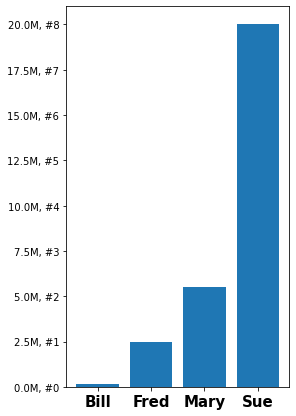
\includegraphics[width=1.22\linewidth]{./gfx/plt-TicksFormatter}
\end{tcolorbox}
%
\end{frame}

% =========================================================================== %

\begin{frame}[fragile]{\LaTeX Elements}
%
\begin{itemize}
\item Labels and Titles may contain (limited) \LaTeX code
\item Encase \LaTeX\xspace elements with \$dollar signs\$
\item Example:
	\begin{itemize}
	\item \inPy{plt.title(r"$\frac {\pi }{2} \approx $ 3.1415")}
	\item Gives $\scriptstyle \frac {\pi }{2} \approx 3.1415$
	\item Prefix r: no escape character (\textbackslash)
	\end{itemize}
\item Possible to use a full scope \LaTeX compiler
	\begin{itemize}
	\item Requires option \inPy{matplotlib.rcParams['text.usetex'] = True}
	\item Requires installed external \LaTeX compiler
	\item Significant runtime
	\end{itemize}
\end{itemize}
%
\end{frame}

% =========================================================================== %

\begin{frame}[fragile]{Plot Elements -- Return Values of the Plot Functions}
%
\begin{itemize}
\item Functions/Methods like \texttt{plot}, \texttt{pie}, ... have return values
\item Represent (collections of) plot elements, \eg lines, wedges, ...
\item Can be used to change Elements dynamically
\item Example:
	\begin{itemize}
	\item \texttt{plt.plot} or \texttt{ax.plot} returns a \inPy{list} of \texttt{Line2D} objects ...
	\item ... which have properties \texttt{data}, \texttt{color}, ...
	\item ... and methods \texttt{set\_color}, etc.
	\item Update only in memory
	\item Update on screen: \texttt{fig.canvas.draw()}
	\end{itemize}
\item See \url{https://matplotlib.org/3.5.0/api/index.html}
\end{itemize}
%
\end{frame}

% =========================================================================== %

\begin{frame}[fragile]
%
\vspace{-5pt}
\begin{codebox}[Code: Updating a Plot]
\begin{minted}[linenos, fontsize=\scriptsize]{python3}
import math
import matplotlib.pyplot as plt

fig = plt.figure()
ax = fig.add_subplot()

X = [x / 100 for x in range(0, 628, 5)]
Y = [math.sin(2 * t) + 2 for t in X]

p = ax.plot(X, Y, "y-", label="foo")
q = ax.plot(X, Y, "r.", label="bar")
fig.show(); input()

print(type(p), p[0], type(p[0]))
# <class 'list'> Line2D(foo) <class 'matplotlib.lines.Line2D'>

print("change red dots to gold dots")
q[0].set_color("gold")

fig.canvas.draw(); input()
\end{minted}
\end{codebox}
%
\end{frame}

% =========================================================================== %

\begin{frame}[fragile]{Text Overlays}
%
\begin{itemize}
\item Put additional free text on screen with command \texttt{plt.annotate} (or method \texttt{ax.annotate}, respectively)
\item Mandatory arguments
	\begin{itemize}
	\item \texttt{text} -- what to print on plot
	\item \texttt{xy} -- \inPy{tuple} of coordinates
	\end{itemize}
\item Optional arguments
	\begin{itemize}
	\item \texttt{xycoords} -- \inPy{str}ing: choice of coordnates
		\begin{itemize}
		\item \inPy{'figure fraction'} -- coordinates between 0 and 1, absolute coordinates (relative to window)
		\item \inPy{'figure pixels'} -- absolute coordinates in pixels
		\item \inPy{'axes pixels'} -- relative to axis of coordinates, unit pixels
		\item \inPy{'data'} (default) -- same coordinates as plot elements
		\end{itemize}
	\item \texttt{horizontalalignment}, \texttt{verticalalignment}
		\begin{itemize}
		\item \inPy{'left'}, \inPy{'center'}, \inPy{'right'}
		\item \inPy{'top'}, \inPy{'center'}, \inPy{'bottom'}
		\end{itemize}
	\end{itemize}
\end{itemize}
%
\end{frame}

% =========================================================================== %

\begin{frame}[fragile]{Text Overlays with Arrows}
%
\begin{itemize}
\item Extended version of \texttt{annotate}
\item Extra parameter \texttt{xytext}
	\begin{itemize}
	\item Sets text position
	\item Again: \inPy{tuple}
	\item \texttt{xy} now is coordinate of tip of arrow
	\end{itemize}
\item Optional argument \texttt{arrowprops}
	\begin{itemize}
	\item \inPy{dict}, specifies look of arrow
	\item see \url{https://matplotlib.org/3.5.0/api/_as_gen/matplotlib.axes.Axes.annotate.html#matplotlib.axes.Axes.annotate}
	\end{itemize}
\end{itemize}
%
\end{frame}

% =========================================================================== %

\begin{frame}[fragile]
%
\begin{codebox}[Example: Annotations, width=.6\linewidth, nobeforeafter, equal height group = grpXmpAnnotate]
\begin{minted}[linenos, fontsize=\scriptsize]{python3}
import math
import matplotlib.pyplot as plt

fig = plt.figure()
ax = fig.add_subplot()

X = [(x - 300) / 100 for x in range(0, 600, 5)]
Y = [math.cos(x*10) * math.exp(-x**2) for x in X]

ax.plot(X, Y)

ax.annotate("Center of Wave Package",
            xy = (0, 1),
            xytext = (0.8, 0.5),
            arrowprops={'arrowstyle' : '->'}
)

plt.show()
\end{minted}
\end{codebox}
%
\begin{tcolorbox}[title=Output: Annotations, width=.34\linewidth, nobeforeafter, equal height group = grpXmpAnnotate]
		
	\vspace{50pt}
	\hspace{-13pt}
	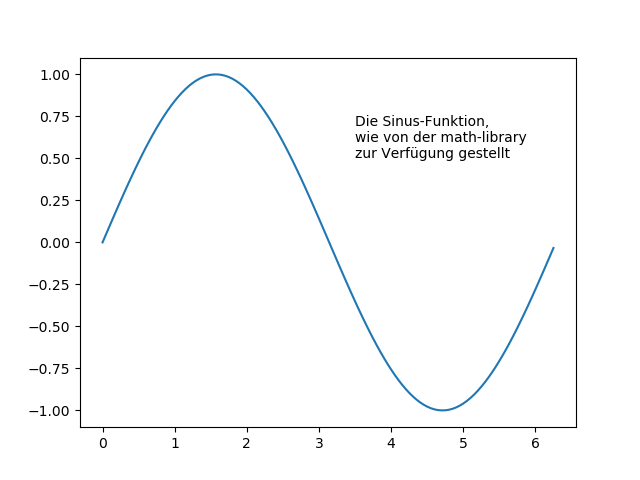
\includegraphics[width=1.22\linewidth]{./gfx/plt-overlay-simple}
\end{tcolorbox}
%
\end{frame}

% =========================================================================== %

\begin{frame}[fragile]{3D Plots}
%
\begin{itemize}
\item Specialized submodule allows 3D plots
\item \inPy{from mpl_toolkits.mplot3d import Axes3D}
\item \inPy{ax = fig.add_subplot(projection='3d')}
\item \texttt{plot} now supports X, Y, Z \Thus curves in 3D
\item Surface plots: \texttt{plot\_wireframe}, \texttt{plot\_surface}
	\begin{itemize}
	\item Requires Numpy module (see next week's lectures)
	\item Preview: \texttt{linspace(start, stop, N)} generates \texttt{N} values between \texttt{start} and \texttt{stop}
	\item Preview: \texttt{meshgrid(iterable1, iterable2, ...)} generates \inPy{tuple}s of all conceivable combinations of the contents of \texttt{iterable1}, ...
	\end{itemize}
\end{itemize}
%
\end{frame}

% =========================================================================== %

\begin{frame}[fragile]
%
\begin{codebox}[Example: 3D Curve, width=.6\linewidth, nobeforeafter, equal height group = grpXmp3DCurve]
\begin{minted}[linenos, fontsize=\scriptsize]{python3}
import math
import matplotlib.pyplot as plt
from mpl_toolkits.mplot3d import Axes3D

fig = plt.figure()
drw = fig.add_subplot(projection='3d')

T = [math.pi * t / 100 for t in range(1000)]
X = [math.exp(-0.05 * t) * math.cos(t) for t in T]
Y = [math.exp(-0.05 * t) * math.sin(t) for t in T]

drw.set_xlabel("x")
drw.set_ylabel("y")
drw.set_zlabel("time t")
drw.set_title("decaying orbit")

drw.view_init(80, 10)   # rotate 80° right, 10° up
drw.plot(X, Y, T)
plt.show()
\end{minted}
\end{codebox}
%
\begin{tcolorbox}[title=Output: 3D Curve, width=.34\linewidth, nobeforeafter, equal height group = grpXmp3DCurve]
	\hspace{-13pt}
	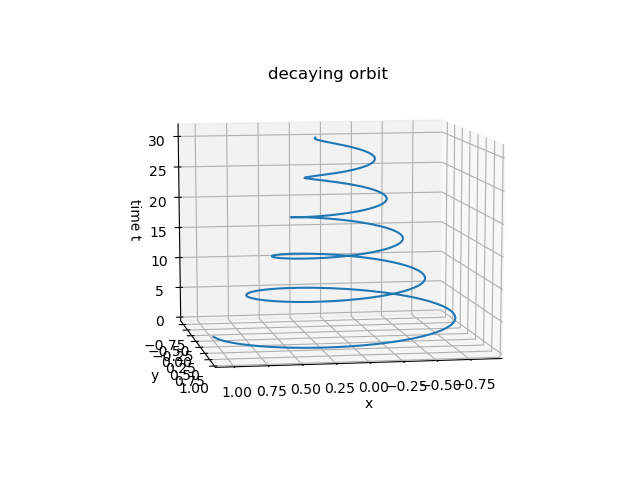
\includegraphics[width=1.22\linewidth]{./gfx/plt-orbit3D}
\end{tcolorbox}
%
\end{frame}

% =========================================================================== %

\begin{frame}[fragile]
%
\begin{codebox}[Example: 3D Surface ..., width=.6\linewidth, nobeforeafter, equal height group = grpXmp3DSurface]
\begin{minted}[linenos, fontsize=\scriptsize]{python3}
import matplotlib.pyplot as plt
from mpl_toolkits.mplot3d import Axes3D
import numpy as np

W = 20
H = 30

func = lambda x, y : x**2 - y**2

X, Y = np.meshgrid(np.linspace(-1.0, 1.0, W),
                   np.linspace(-1.5, 1.5, H))
Z = X**2 - Y**2

fig = plt.figure( figsize=(4,8) )
ax1 = fig.add_subplot(211, projection='3d')
ax2 = fig.add_subplot(212, projection='3d')

ax1.plot_wireframe(X, Y, Z)
ax2.plot_surface  (X, Y, Z)

plt.show()

\end{minted}
\end{codebox}
%
\begin{tcolorbox}[title=Output: 3D Surface, width=.34\linewidth, nobeforeafter, equal height group = grpXmp3DSurface]
	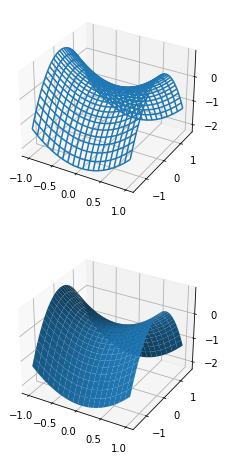
\includegraphics[width=.9\linewidth]{./gfx/plt-surface3D}
\end{tcolorbox}
%
\end{frame}

% =========================================================================== %

\begin{frame}[fragile]{Pseudo 3D Plots}
%
\begin{itemize}
\item Personal opinion: 3D plots are fancy but hard to read
\item Elements hidden behind peaks
\item My preference: colour maps
\item \texttt{plt.pcolor}
	\begin{itemize}
	\item One rectangle per data point
	\end{itemize}
\item \texttt{plt.contour}
	\begin{itemize}
	\item Contour plot
	\item Lines with (interpolated) same z coordinate
	\end{itemize}
\item \texttt{plt.contourf}
	\begin{itemize}
	\item Same as \texttt{contour}, but filled areas
	\end{itemize}
\item For all
	\begin{itemize}
	\item Available as command and as method on \texttt{ax}
	\item Optional parameter \texttt{cmap} specifies a Colourmap
	\item See \url{https://matplotlib.org/stable/gallery/color/colormap_reference.html}
	\end{itemize}
\end{itemize}
%
\end{frame}

% =========================================================================== %

\begin{frame}
%
\begin{tcolorbox}[title=Pseudo 3D Plots]
	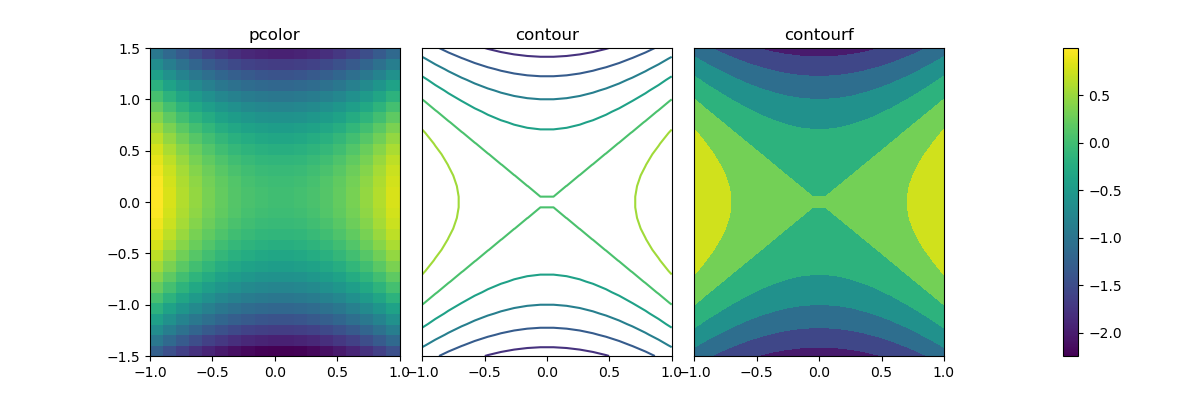
\includegraphics[width=\linewidth]{./gfx/plt-falseColour}
	
	\scriptsize
	Plots generated from same arrays \texttt{X, Y, Z} as before.
\end{tcolorbox}
%
\end{frame}

% =========================================================================== %

\begin{frame}[fragile]
%
\begin{codebox}[Code: Pseudo 3D Plots]
\begin{minted}[linenos, firstnumber=last, fontsize=\scriptsize]{python3}
# same X, Y, Z as before
fig = plt.figure(figsize=(12,4)); grd = fig.add_gridspec(1, 7)

pcl = fig.add_subplot(grd[0,0:2]); pcl.set_title("pcolor")
col = pcl.pcolor(X, Y, Z, shading='auto')

cnt = fig.add_subplot(grd[0,2:4]); cnt.set_title("contour")
cnt.set_yticks([])
cnt.contour(X, Y, Z)

cnf = fig.add_subplot(grd[0,4:6]); cnf.set_title("contourf")
cnf.set_yticks([])
cnf.contourf(X, Y, Z)

bar = fig.add_subplot(grd[0,6]); bar.axis("off")
fig.colorbar(col)
plt.show()
\end{minted}
\end{codebox}
%
\end{frame}

% =========================================================================== %

\begin{frame}[fragile]{Saving Plots to the Hard Disk}
%
\begin{itemize}
\item Objects of type \texttt{Figure} have method \texttt{savefig}
\item Mandatory argument: \inPy{str}ing filename
\item Optional Parameters
	\begin{itemize}
	\item \texttt{format}: \inPy{str}ing, specifies file format (\eg \inPy{'png'}, \inPy{'jpg'}, \inPy{'svg'}, \inPy{'pdf'}, ...).\\
		Deduced from filename if omitted
	\item \texttt{facecolor}: background colour of the file output
	\item \texttt{edgecolor}: border color of the file output
	\item \texttt{transparent}: \inPy{bool} makes plot background transparent
	\item See \url{https://matplotlib.org/3.5.0/api/figure_api.html?highlight=savefig#matplotlib.figure.Figure.savefig}
	\end{itemize}
\end{itemize}
%
\end{frame}
\end{document}

% MAREI!!
% whom do I give credit? Where?